\chapter{Návrh systému pro infračervený přenos dat}
\zkratka{LG} je založeno na optickém přenosu dat ze zbraně do vesty. Tato data jsou naprosto klíčová, nesou v sobě informace o tom, kdo je vyslal a chyba při přenosu nebo interpretaci těchto dat, by byla fatální. V nejhorším případě by mohla způsobit přičtení bodů špatnému hráči, což by poškodilo střelce a při kumulaci těchto chyb by \zkratka{LG} hráče brzy omrzela. Proto je potřeba se problematikou optického přenosu dat zabývat.

Při \zkratka{LG} jsou data přenášena v infračerveném pásmu elektromagnetických vln, což odpovídá vlnovým délkám $\lambda \in \langle 760~\jedn{nm};~1~\jedn{mm}\rangle$. Tyto vlnové délky jsou pro lidské oko nedetekovalné a tak si běžný hráč přenášených dat, ani nevšimne.

\section{Požadavky na systém}
Sytém musí být schopen vyslat po stisknutí spouště, informace o tom kdo vystřelil. Tyto informace musí být také schopen přijmout, dekódovat a rozhodnout jestli jsou data vpořádku nebo přišla poškozená. Data by měla být schopna adresovat minimálně 12 hráčů a čas od výstřelu do vyhodnocení dat co nejratší aby nedošlo k tomu, že hráč vystřelí někoho zastřelí a on by mohl ještě několik okmažiků hrát.

\section{Návrh přenášeného packetu}
Rozhodl jsem se použít osm bitů pro adresu a šestnáct bitů pro kontrolním součet. Takto vzniklí adresovací prostor pokryje všechny hráče s dostatečnou rezervou pro možné rozšíření systému o interaktivní překážky. Hráči ubdou adresování od nuly do $n$, kde $n = počet _{hráčů} - 1$.

\begin{figure}[H]
    \begin{center}
        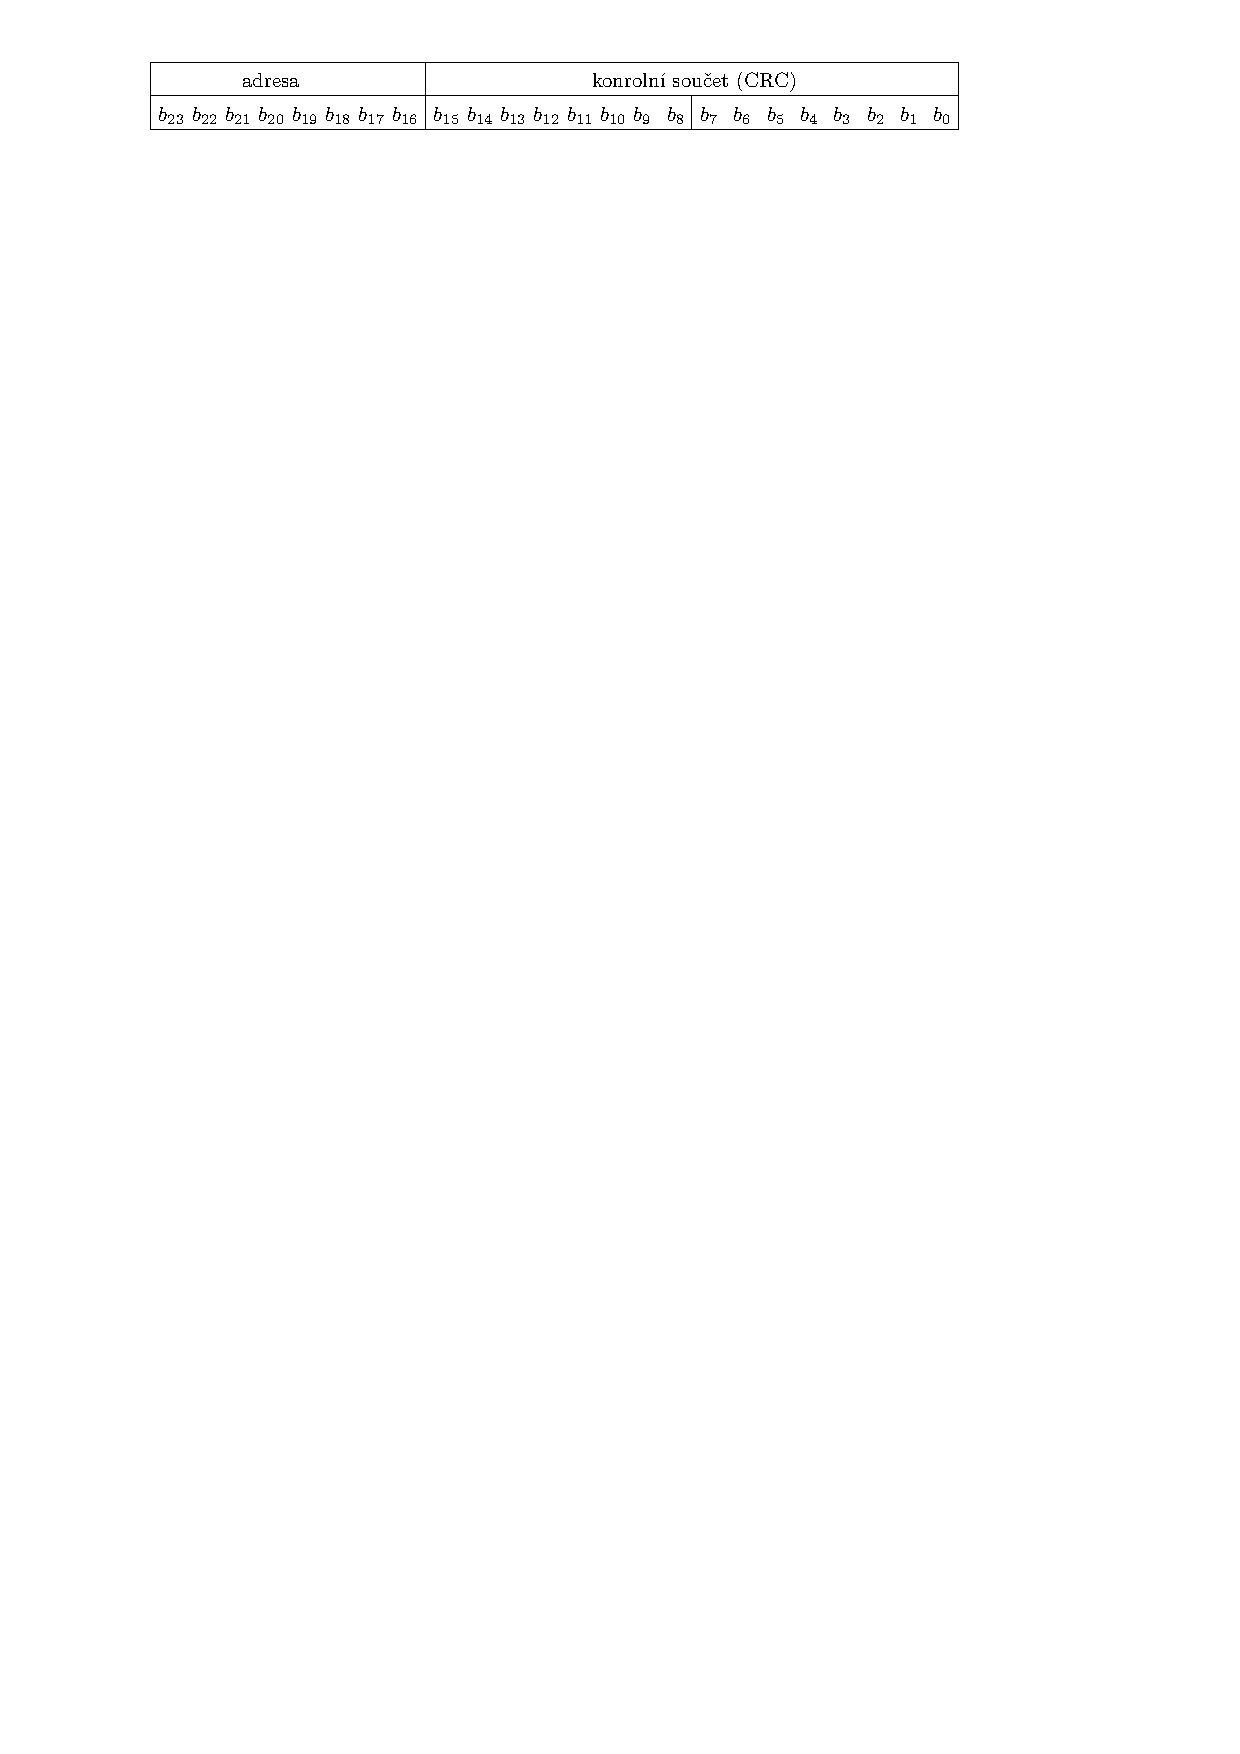
\includegraphics[width=\textwidth]{img/ir-packet}
    \end{center}
    \caption{Obrázek struktury packetu}
\end{figure}

\section{Výběr IR vysílače}
IR vysílač má za úkol v relativně širokém rozsahu zvdáleností (přibližně 1 až 15 metrů) zasáhnou zásahové čidlo a předat mu informaci o tom, kdo jej zasáhl.

S dostupných součástek na trhu, jsem se snažil najít kompromis mezi cenou, výkonem a vyzařovacím úhlem.

IR lasery se při laser game příliš často nepoužívají, protože jejich paprsek je velmi úzký a nevytvořil by se kužel o dostatečném průměru, který by zasahovl hráče. Laser by se se musel doplnit dodatečnou optikou, což by vyžadovalo další náklady. Proto se pro přenos dat využívají IR LED. U těchto diod je třeba vyřešit problém zcela opačný a to je vybrat LED s dostatečně malým vyzařovacím úhlem.

Při experimetech s IR LED s různými vyzařovacími úhly, se mi pro tento účel jevili jako ideální diody s vyzařovacím úhlem $12^\circ$, vložené do $10$~\jedn{cm} trubičky. Diody s menším vyzařovacím úhlem byli problematické při malích vzdálenostech, protože vyzařovaný kužel byl příliš malý.

Důleživým parametrem IR LED je vlnová délka vyzařovaného záření. Její volba závisí na použitém přijímači. Pokud by měli vysílač s přijímačem rozdílnou vlnovou délku, nastával by útlum signálu, tím větší čím větší by byl rozdíl vlnových délek. Proto jsem si vybral jednu z nejvíce vyráběný vlnovových délek $940~\jedn{nm}$.

\section{Výběr IR přijímače}
IR přijímač má za úkol detekovat IR záření vysílané vysílačem. Vzhledem k tomu že přijímače jsou integrované přímo ve vestě je důležitým kritériem jejich velikost. Integrované přijímače jsou pro tento úřel ideální. mají v sobě integrovanou fotodiodu, vstupní transimpedančí zesilovač, pásmovou propust, demodulátor i zesilovač, který má nastavitelné zesílení a snaží se udržet amplitudu výstupního signálu stabilní. Navíc většina těchto zesilovačů má výstup typu otevřená kolektor, takže jsou snímače spojovat bez nutnosti použít další součástky jako třeba diody.

Klíčovým parametrem je snímací úhel, v případě snímačů by bylo odeální, kdyby snímali záření dopadající i pod úhlem $90^\circ$ stejně citlivě jako záření dopadající na snímač přímo pod nulovým úhlem. Takoví snímače ale nejsou dostupné. Snímače které jsou na trhu mají nejšastěji přijímací úhel $45^\circ$, pro použití při laser game je ale ale málo, tak jsem našel přijímač OSRB38C9BA s úhlem $90^\circ$ a vlnovou délkou $940~\jedn{nm}$.

\begin{figure}[H]
    \begin{center}
        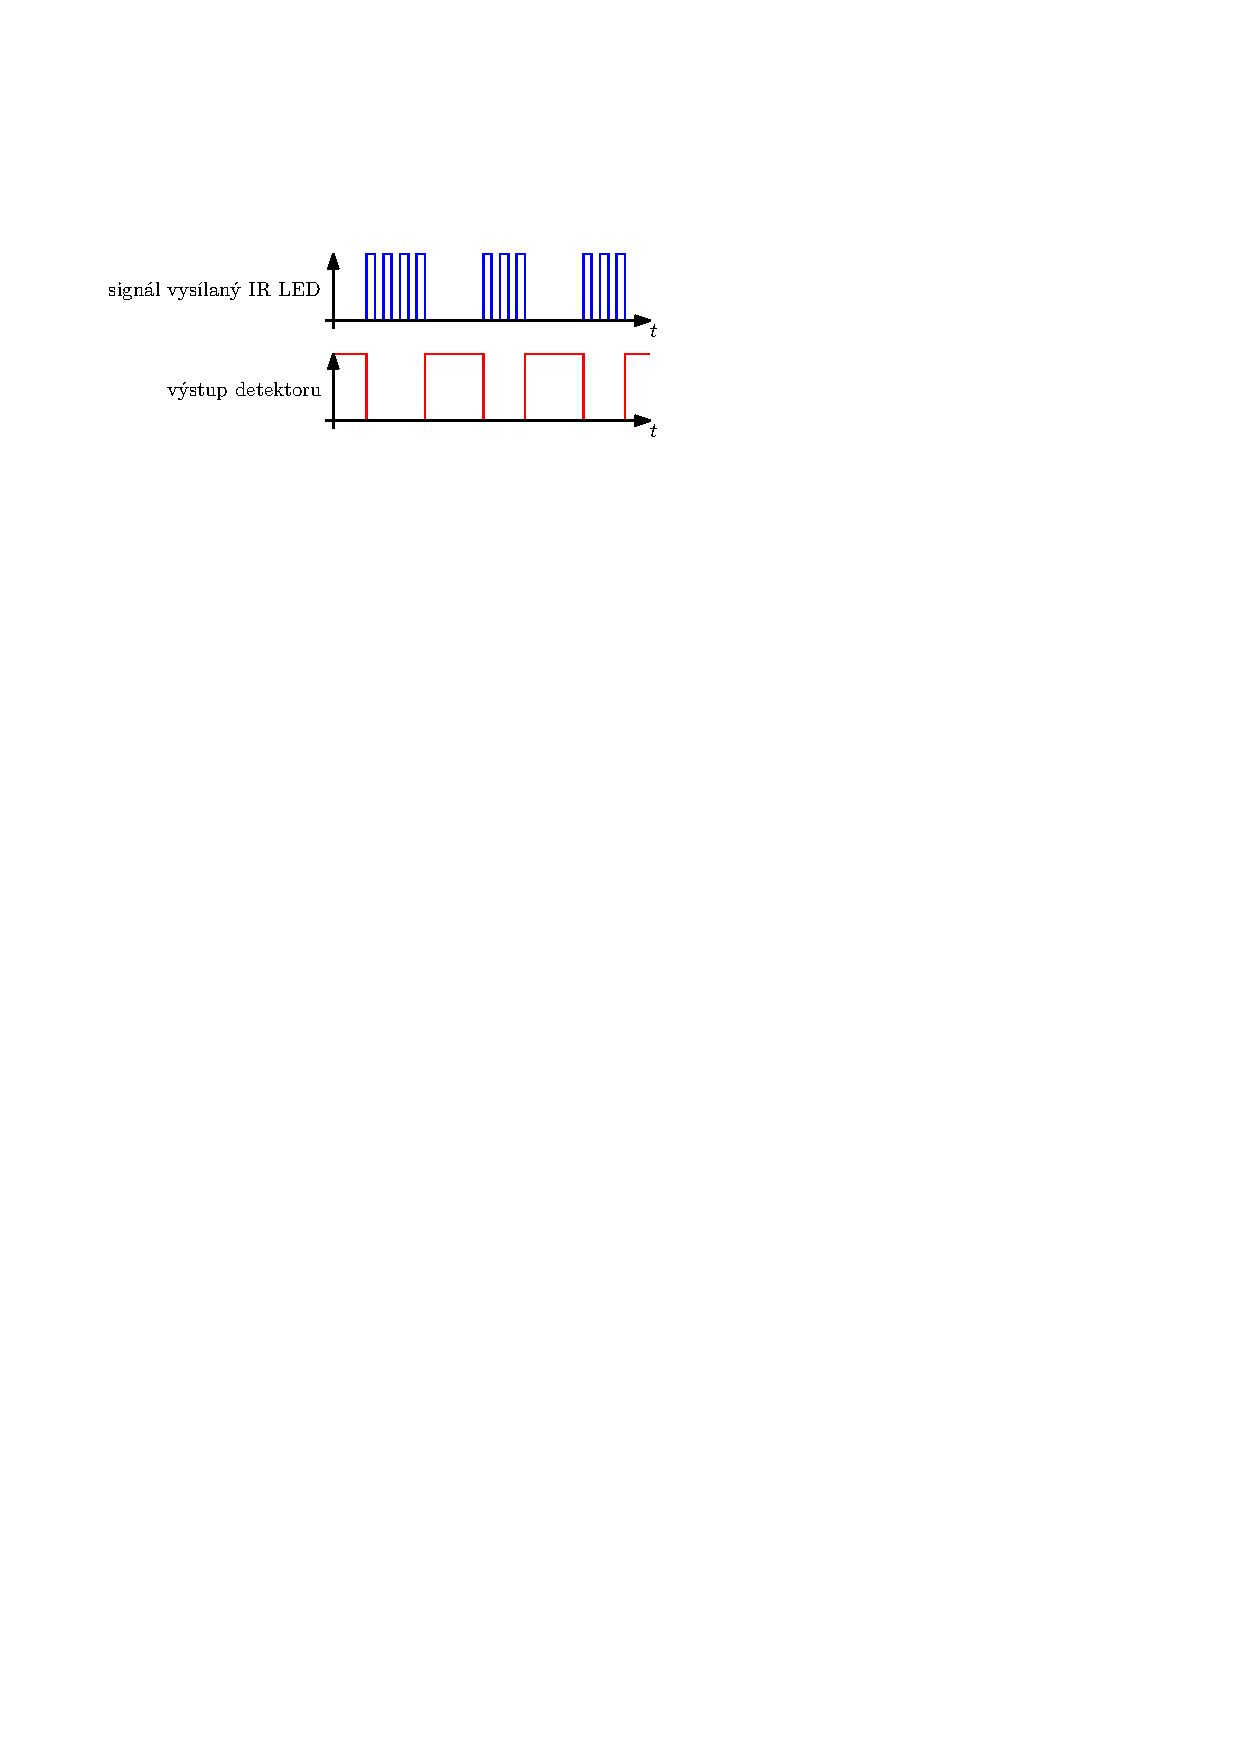
\includegraphics[width=0.7\textwidth]{img/funkce-ir-detektoru}
    \end{center}
    \caption{Ukázka funkce ideálního integrovaného detektoru}
\end{figure}

Tento přijímač očekává signál modulovaný na nosný signál $37,9~\jedn{kHz}$. Důležitou vlastrností přijímače je tolerance výstupního signálu $\pm 200~\jedn{\mikro s}$ na vstupní testovací puls o šířce $600~\jedn{\mikro s}$.

\section{Přenos IR signálu}
IR signál je přenášen od vysílače vzduchem k přijímači. IR signál má vlastnost, že se dobře odráží od bílích stěn, toho lze pozorovat například na ovladačích ke spotřební elektronice, ktré fungují na stejných principech, pokud ovladač namíříme na bílí strop IR zíření se od něji odrazí a dostane se až k detektoru spotřebiče. Proto jsou stěny v LG arénách tmavé, aby záření pohlcovali.

Přenášený IR signál musí být modulovaný na nosnou vlnu. Pokud by nebyl modulovaný, stačilo by na detektor jen posvítit například ze zářivky a detektor by toto záření intepretoval jako náš požadovaný signál, přestože by se jednalo o rušení.Takto náhodně generované rušení může oklamat i CRC. Bohužel, namodulování signálu na nosnou vlnu nezabrání všemu rušení do systému proniknout. Už jsem se setkal s LED osvětlením, které mělo spínaný měnič právě na frekvenci nosné a můj systém rušilo. Proto je důležité v LG aréné používat kavalitní světlené zdroje s měniči pracujícími na vyšších frekvencích.

\section{První návrh systému IR přenosu dat}
\begin{figure}[H]
    \begin{center}
        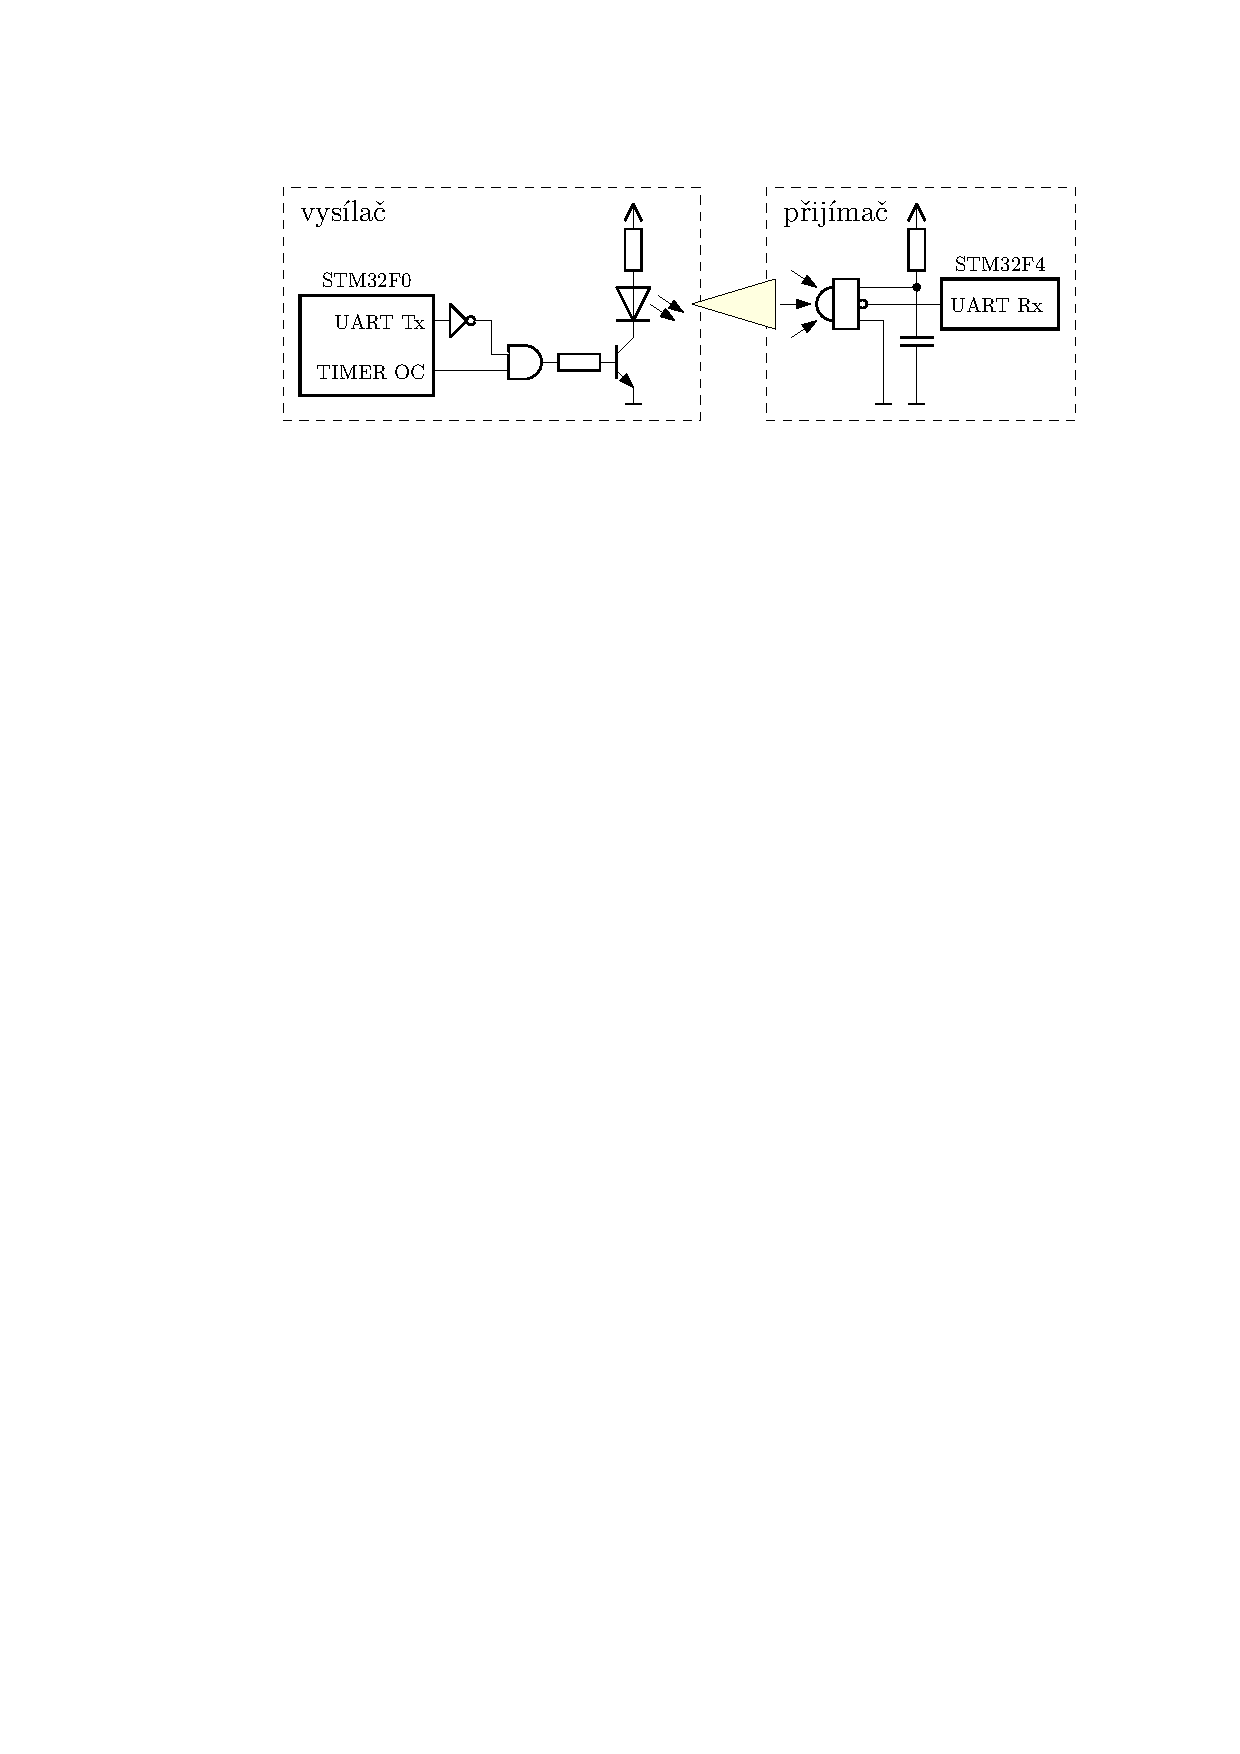
\includegraphics[width=\textwidth]{img/fake}
    \end{center}
    \caption{Zjednodušené schéma první verze systému pro IR přenos dat}
\end{figure}

\subsection{Vysílač}
Vysílač je založen na modulování \zkratka{UART} na \zkratka{PWM}. PWM generuje mikrokontrolér. Frekvence PWM je nakonfigurována na hodnotu $37,9~\jedn{kHz}$, protože na ni má IR detektor největší zisk. Změna střídy nastavuje dosvit vysílače.

Protože UART má klidový stav v logické jedničce, tak je invertován pomocí hradla NOT, a pomocí hradla AND namodulován na PWM. Kdyby nebyl invertovanán tak by vysílací LED většinu času strávila vysíláním, coč by zbytečně zvětšilo spotřebu a navíc by mohlo dojít k zahlčení detektoru.

\subsection{Přijímač}
Přijímač k dekódování přijatého signálu využívá UART integrovaný v mikrokontroléru. Klidový stav detektoru je díky integrovanému pull-up odporu v logické jedničce, pokud detekuje signál, tak stáhne výstup do logické nuly. Tohle chování detektoru je pro nás vhodné protože vysíláme pouze nulové bity. Detektor je opatřen RC článkem paby do něj nevnikalo rušení z napájecího vedení.

UART byl nastaven na přenosovou rychlost $2400~\jedn{bps}$. Na jeden bit trvá přibližně $416~\jedn{\mikro s}$. Perioda jednoho PWM pulzu je $23~\jedn{\mikro s}$, tedy na jeden bit připadá $16$ PWM pulzů. Vzhledem k toleranci detektoru je patrná pčíčina vzniká chyb při zahlcení, zkrátka přenosová rychlost je na použitý detektor příliš vysoká. Experimentálěn jsem vyzkoušel i nejnižší standardní přenosovou rychlost $1200~\jedn{bps}$. Jeden bit tedy trval $832~\jedn{\mikro s}$. Ale stále při posílání dat s lekým počtem nul docházelo velmi často k chybám. Mohl bych ještě snižovat přenosovou rychlost, ale neomezil bych tím zahlcování detektorů, proto jsem se rozhodl navrhnout vlatní komunikační protokol.

\subsection{Zhodnocení systému}
Tento koncepce není moc spolehlivý. Pokud se vysílají data, která obsahují velké množství nul, po několika paketech dojde k zahlcení detektoru. To se projevuje tak, že se projevý tolerance detektoru $\pm200~\jedn{\mikro s}$, která deformuje přijímaný signál. UART tyto data podé dekóduje s velkou chybovostí. Díky CRC kontorle se sice vyhodnotí, že data jsou chybná, tudíž nedojde k usmrcení zasařeného hráče a přičtení bodů špatnému hráči, ale pokud hřáč protihráče zasáhl a on přesto žije, kazí to hru. Pokud se přeručí část packetu (poslední byte) při přenosu, UART tuto chybu neodhalí a od přerušení spojení nabyte zbytek bitů hodnotu jedna.


\section{Druhý návrh systému IR přenosu dat}

\begin{figure}[H]
    \begin{center}
        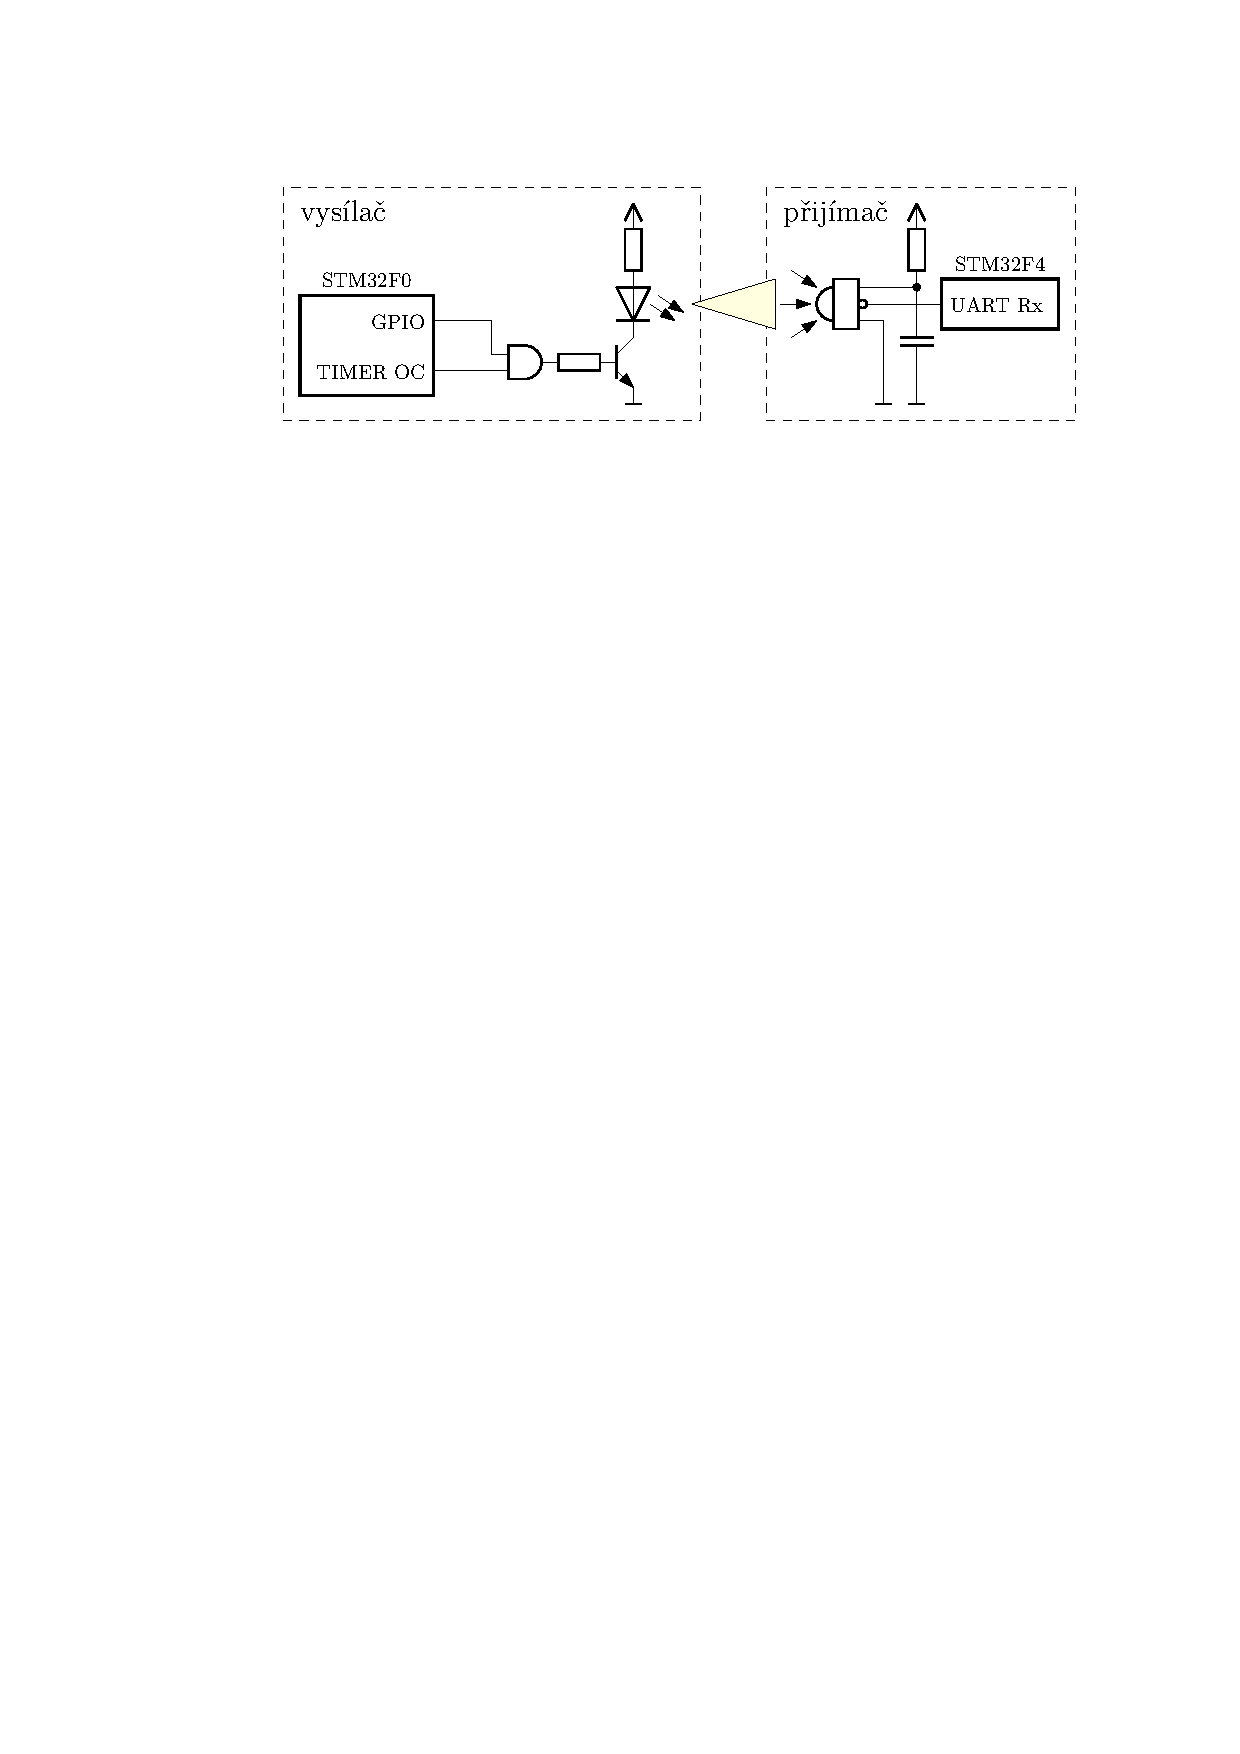
\includegraphics[width=\textwidth]{img/ir-system}
    \end{center}
    \caption{Zjednodušené schéma druhé verze systému pro IR přenos dat}
\end{figure}

Tento systém, vzniknul jako náhrada systému předchozího. Je navržen tak, aby odolával problémům se shnulky nul a korektně dekódovat data i při jejich deformaci o $\pm200~\jedn{\mikro s}$.

Systém už není založen na modulování UARTu na PWM signál. Byl inspirován komunikačními protokoly dálkových ovladačů, které jsou robustní a spolehlivé. Pro přenos jsem si navrhnul vlastín komunikační protokol. Jak jednička tak nula jsou reprezentovány pulzem a charakteristickou mezerou, takže pokud dojde k ke strátě části packetu, problém je odhalen, protože bude porušen komunikační protokol.

\subsection{Komunikační protkokol}
Komunikace začíná odesláním startovacího impulzu, poté následuje startovací mezera. Po této sekvenci následuje 24 period zečínajících vždy datovým pulsem, který má pevnou délku, následovaným mezerou, která definuje zda-li se přenáší jednička, nebo nula. Po dokončení posílání datových bitů následuje ukončovací pulz. Jednotlivé packety jsou od sebe navíc odděleni mezerou, která má definovanou minimální délku. Při vyhodnocování se počítá s tolerancí $\pm250~\jedn{\mikro s}$, čož s rezervou pokryje toleranci optického přijímače.

\begin{table}[H]
  \caption{Definice časování kominikačního protokolu}
  \begin{center}
  	\small
	  \begin{tabular}{|l|r|}
	    \hline
	    \textbf{název} & \textbf{čas [\jedn{\mikro s}]} \\\hline\hline
	    \texttt{IR\_TIM\_START\_PULS}       &  5000     \\\hline
	    \texttt{IR\_TIM\_START\_SPACE}      &  5000     \\\hline
	    \texttt{IR\_TIM\_DATA\_PULS}        &   600     \\\hline
	    \texttt{IR\_TIM\_DATA0\_SPACE}      &   600     \\\hline
        \texttt{IR\_TIM\_DATA1\_SPACE}      &  1200     \\\hline
        \texttt{IR\_TIM\_END\_PULS}         &  3000     \\\hline
        \texttt{IR\_TIM\_PACKET\_SPACE}     & 30000     \\\hline
        \texttt{IR\_TIM\_TOLERANCE}         &   250     \\\hline
	  \end{tabular}
  \end{center}
\end{table}



\subsection{Zhodnocení}
Tento protokol je spolehlivý, povedlo se jím opravit všechny nedostatky, kterými trpěla předchozí verze. Navíc došlo k zjednodušenění HW. V přijímači už není potřeba mít hradlo NOT. Z HW by se mohlo vypustit i hradlo AND a nahrhradit jej hradlem NAND, které je součástí IRTIM (IR timeru, který vznikne spojením timeru 16 a 17) integrovaným přímo v některých STM32F0 mikrokontrolérech. Nakonec ale pro vysílač stačlo použít malý mikrokontorlér STM32F042F6P6, takže použít diskrétníhradlo AND bylo nezbytné.

Maximální doba přnosu jednoho packetu (plného jedniček), trvá $86,2~\jedn{ms}$. Minimální dopa přenosu packetu (plného nul) je $71,8~\jedn{ms}$. Maximální přenosová rychlost je $334~\jedn{bps}$. Minimální přenosová rychlost je $278~\jedn{bps}$. Dosažené přenosové rychlosti jsou sice mnohem nižší než v předchozí verzi, ale vzhledem k přenšenému oběmu dat $24~\jedn{b}$ po stisku souště je doba přenosu přijatelná.

Pokud by bylo potřeba, protokol někdy upravit, tak přenosová rychlost jde navýšit, snížením rozestupu mezi packety.


\begin{figure}[H]
    \begin{center}
        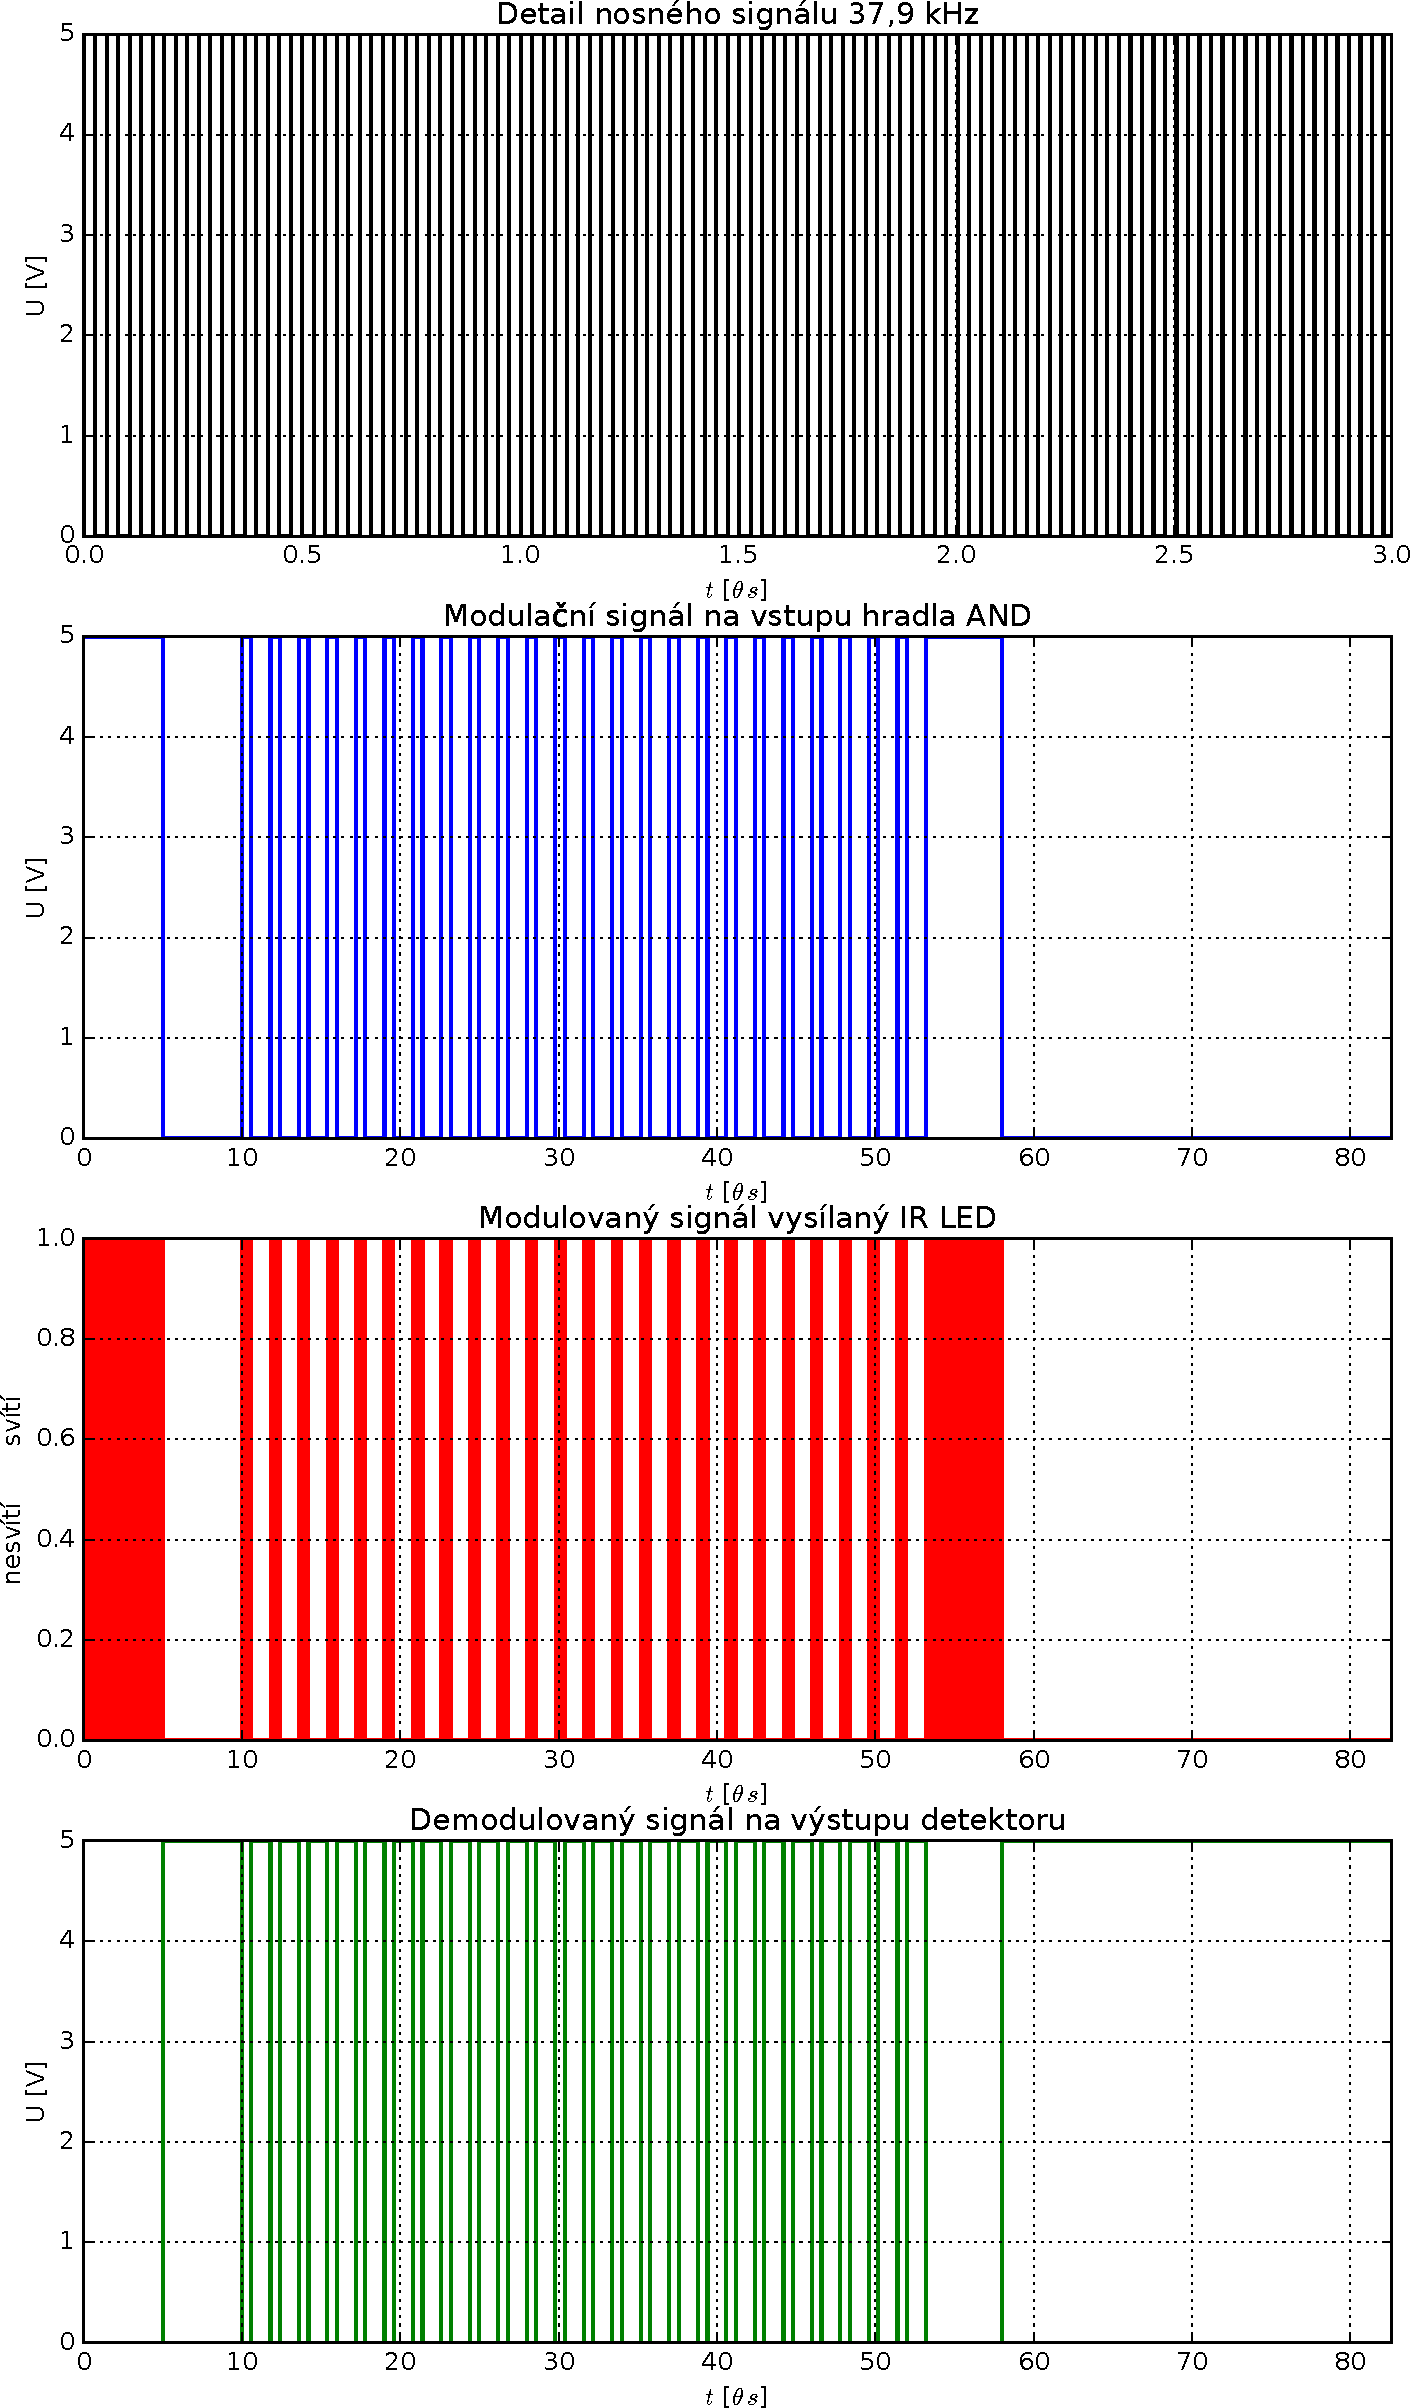
\includegraphics[height=0.97\textheight]{img/model-ir-komunikace}
    \end{center}
    \caption{simulace časových průběhů komunikačního protokolu při přenosu nulového packetu}
\end{figure}
